% DO NOT COMPILE THIS FILE DIRECTLY!
% This is included by the other .tex files.

\begin{frame}[t,plain]
\titlepage
\end{frame}

%\begin{frame}{Índice}
%	\tableofcontents
%\end{frame}

\section{Tumor model}

\begin{frame}{Cahn-Hilliard equation}
	\begin{block}{}
		\vspace*{-0.2cm}
		\begin{equation*}
			\begin{aligned}
				u_t&= \nabla\cdot \left(M(u)\nabla\mu\right)\quad&\text{in }\Omega\times(0,T),\\
				\mu&=-\varepsilon^2\Delta u+F'(u)\quad&\text{in }\Omega\times(0,T),\\
				\nabla u\cdot \mathbf{n}&=\nabla(-\varepsilon^2\Delta u+F'(u))\cdot\mathbf{n}=0\quad&\text{on }\partial\Omega\times(0,T),\\
				u(0)&=u_0\quad&\text{in }\Omega.
			\end{aligned}
		\end{equation*}
	\end{block}
	\begin{itemize}
		\item $\alert{F(u)}=\frac{1}{4}u^2(1-u)^2$ Ginzburg-Landau double well functional.
		\item $\alert{M(u)}=u_\oplus(1-u)_\oplus$ degenerate mobility function.
		\begin{itemize}
			\item $v_\oplus \coloneqq\max\{v,0\}$,\quad
			$v_\ominus \coloneqq-\min\{v,0\},$\quad
			$v=v_\oplus  - v_\ominus$.
		\end{itemize}
		\item $u$ \structure{minimizes energy functional}:
		$$\alert{E(u(t))}\coloneqq\frac{\varepsilon^2}{2}\int_\Omega|\nabla u(t)|^2dx+\int_\Omega F(u(t))dx.$$
		\item Pointwise bounds: $u\in[0,1]$. 
	\end{itemize}
\end{frame}

\subsubsection{Tumor model}
\begin{frame}{Tumor model}
	\begin{block}{}
		\begin{center}
			\structure{\textbf{Cahn-Hilliard model (\alert{tumor})}} \alert{+} \structure{\textbf{Diffusion equation (\alert{nutrients})}}
		\end{center}
	\end{block}
	\begin{figure}[h!]
		\centering
		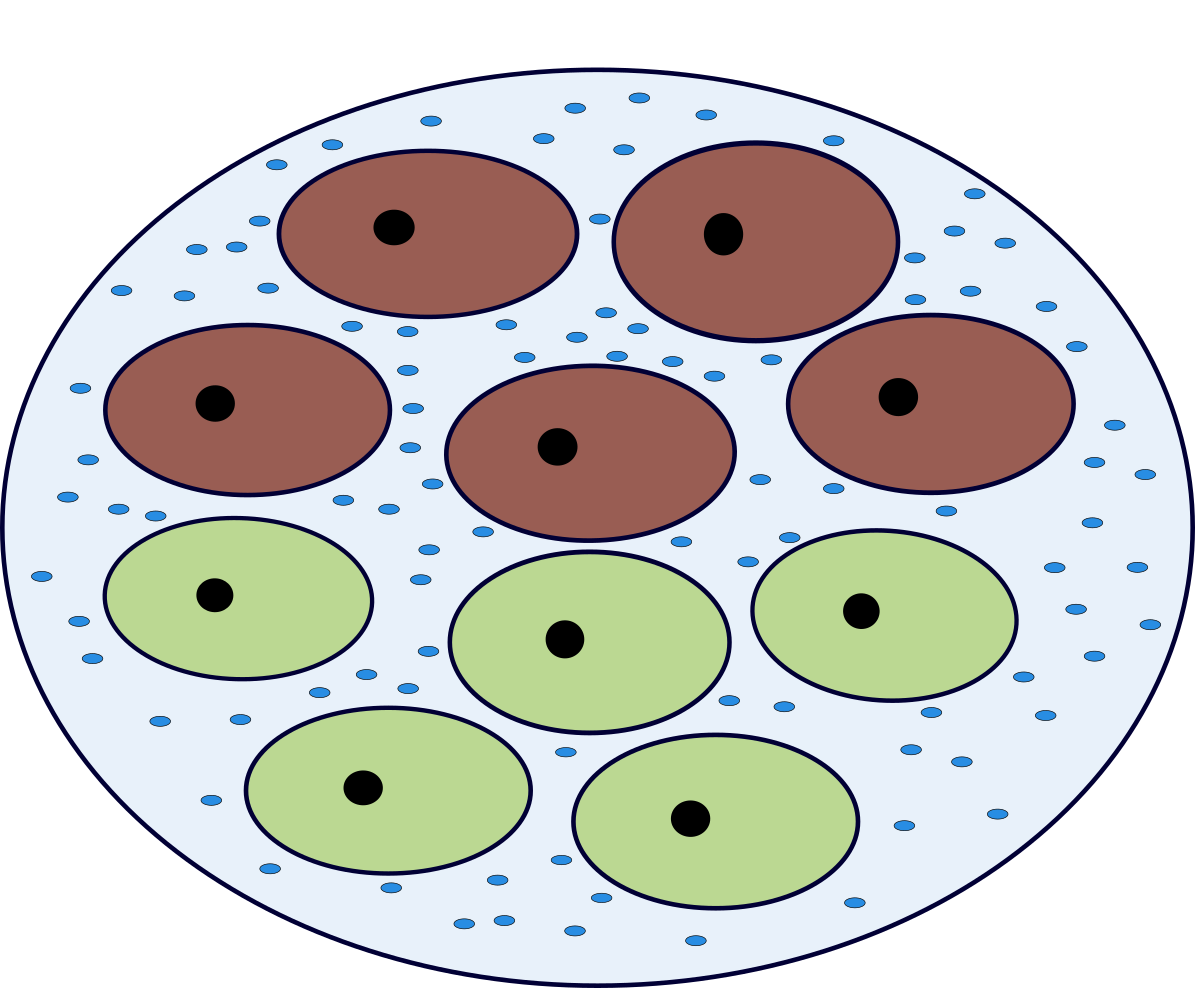
\includegraphics[scale=0.1]{img/celulas.png}
		\caption{Interaction between the four species.}
	\end{figure}
	Variables $\alert{u}$ and $\alert{n}$ bounded on $[0,1]$:
	\begin{itemize}
		\item $\alert{u}$ phase-field variable ($1$ tumor cells and $0$ healthy cells).
		\item $\alert{n}$ nutrient-rich extracellular water volume fraction.
	\end{itemize}

	
	%	\structure{\textbf{energía}} $E\colon H^1(\Omega)\times H^1(\Omega)\longrightarrow\R$ se define como 
	%	\begin{align*}
		%	E(u(t),n(t))&\coloneqq\int_\Omega\left(\frac{\varepsilon^2}{2}|\nabla u(x,t)|^2+F(u(x,t))-\chi_0u(x,t)n(x,t)+\frac{1}{2\delta}\left(n(x,t)\right)^2\right)dx.
		%	\end{align*}
\end{frame}

\begin{frame}{Tumor model {\footnotesize (derived from \cite{van_der_zee_model})}}
	\footnotesize
	\vspace*{-0.2cm}
	\begin{block}{}
		\vspace*{-0.4cm}
		\begin{subequations}
			\begin{align*}
				\partial_t u&=C_u\nabla\cdot\left(M(u)\nabla\mu_u\right)+\framedmath<2>{\delta P_0P(u,n)(\mu_n-\mu_u)_\oplus} \quad&\text{in }\Omega\times (0,T),\\
				\mu_u&=F'(u)-\varepsilon^2\Delta u\framedmath<3>{-\chi_0 n}\quad&\text{in }\Omega\times (0,T),\\
				\partial_t n&=C_n\nabla\cdot\left(M(n)\nabla\mu_n\right)-\framedmath<2>{\delta P_0P(u,n)(\mu_n-\mu_u)_\oplus} \quad&\text{in }\Omega\times (0,T),\\
				\mu_n&=\frac{1}{\delta} n \framedmath<3>{-\chi_0 u} \quad&\text{in }\Omega\times (0,T),\\
				\nabla u\cdot \mathbf{n}&=\left( M(n)\nabla \mu_n\right)\cdot \mathbf{n}=\left( M(u)\nabla \mu_u\right)\cdot \mathbf{n}=0 \quad &\text{on }\partial\Omega\times (0,T),\\
				u(0)&=u_0,\quad n(0)=n_0\quad&\text{in }\Omega,%\\
				%\mu_u(0)&=f'(u_0)-\varepsilon^2\Delta u_0-\chi_0 n_0\quad&\text{en }\Omega,
			\end{align*}
		\end{subequations}
	\end{block}
	where $u_0,n_0\in L^2(\Omega)$are the initial conditions.
	
	\vspace*{0.2cm}
	\begin{itemize}
		\item $M(v)\coloneqq h_{p,q}(v)$, $P(u,n)\coloneqq h_{r,s}(u)n_\oplus$ where 
		$$
		h_{p,q}(v)\coloneqq K_{p,q}v_\oplus^p(1-v)_\oplus^q
		$$
		with $K_{p,q}>0$ a constant so that $\max_{x\in\R}h_{p,q}(v)=1$.
		\item<2> \myframed{Cells-nutrients chemical reactions.}
		\item<3> \myframed{Movement of tumor cells $\longleftarrow$ \textbf{Cross-diffusion terms}.}
	\end{itemize}	
\end{frame}

\begin{frame}{Properties of the model}
	\begin{proposition}
		Let $u_0,v_0\in[0,1]$, then $u(t),n(t)\in[0,1]$ for a.e. $t\in(0,T)$.
	\end{proposition}
	\begin{proposition}
		The total mass of tumor cells and nutrients is conserved: $$\frac{d}{dt}\int_\Omega (u(x,t)+n(x,t))dx=0.$$
	\end{proposition}
\end{frame}
\begin{frame}{Properties of the model}
	\scriptsize
	\begin{proposition}
		If $\partial_t u\in L^2(0,T, H^1(\Omega))$, then it satisfies the following energy law
		\begin{align*}
			\frac{d E(u(t),n(t))}{dt}&+C_u\int_\Omega M(u(x,t))|\nabla\mu_u(x,t)|^2dx+C_n\int_\Omega M(n(x,t))|\nabla\mu_n(x,t)|^2\notag\\&+\delta P_0\int_\Omega P(u(x,t),n(x,t))(\mu_u(x,t)-\mu_n(x,t))_\oplus ^2dx=0,
		\end{align*}
		where
		\begin{align*}
			E(u(t),n(t))&\coloneqq\int_\Omega\left(\frac{\varepsilon^2}{2}|\nabla u(x,t)|^2+ F(u(x,t))-\chi_0u(x,t)n(x,t)+\frac{1}{2\delta}\left(n(x,t)\right)^2\right)dx.
		\end{align*}
		Therefore, the solution is energy stable in the sense $$\frac{d}{dt}E(u(t),n(t))\le 0.$$
	\end{proposition}
\end{frame}

\section{Approximation of the model}
\begin{frame}{FE and DG methods}
	\footnotesize
	\vspace*{-0.2cm}
	\begin{block}{}
		\text{Finite Element method:}
		\begin{equation*}
			\alert{\Pc_k(\T_h)}\coloneqq\left\{v_h\in \mathcal{C}^0(\overline\Omega)\colon v_{h|_{K_i}}\in\mathbb{P}_k(K_i)\text{ with } K_i\in\T_h,\forall i\in\left\{1,2,\ldots,N_{\T_h}\right\}\right\},
		\end{equation*}
		\text{Discontinuous Galerkin method:}
		\begin{equation*}
			\alert{\Pd_k(\T_h)}\coloneqq\left\{v_h\in L^2(\Omega)\colon v_{h|_{K_i}}\in\mathbb{P}_k(K_i)\text{ with } K_i\in\T_h,\forall i\in\left\{1,2,\ldots,N_{\T_h}\right\}\right\},
		\end{equation*}
	\end{block}
	with a basis $\left\{\phi_i\right\}_{i\in\left\{1,2,\ldots,N_h \right\}}$.
	
	\vspace*{0.3cm}
	Notation:
	
	\begin{minipage}{0.69\textwidth}
	\begin{itemize}
		\item \structure{Average}: 
		$\alert{\media{v}}\coloneqq
		\begin{cases}
			\dfrac{\vK+\vL}{2}&\text{if } e=\partial K\cap\partial L\in\E_h^i\\
			\vK&\text{if }e=\partial K\in\E_h^b
		\end{cases},$
		\item \structure{Jump}: $
		\alert{\salto{v}}\coloneqq
		\begin{cases}
			\vK-\vL&\text{if } e=\partial K\cap\partial L\in\E_h^i\\
			\vK&\text{if }e=\partial K\in\E_h^b
		\end{cases},$
	\end{itemize}
	\end{minipage}
	\begin{minipage}{0.29\textwidth}
		\begin{figure}
			\centering
			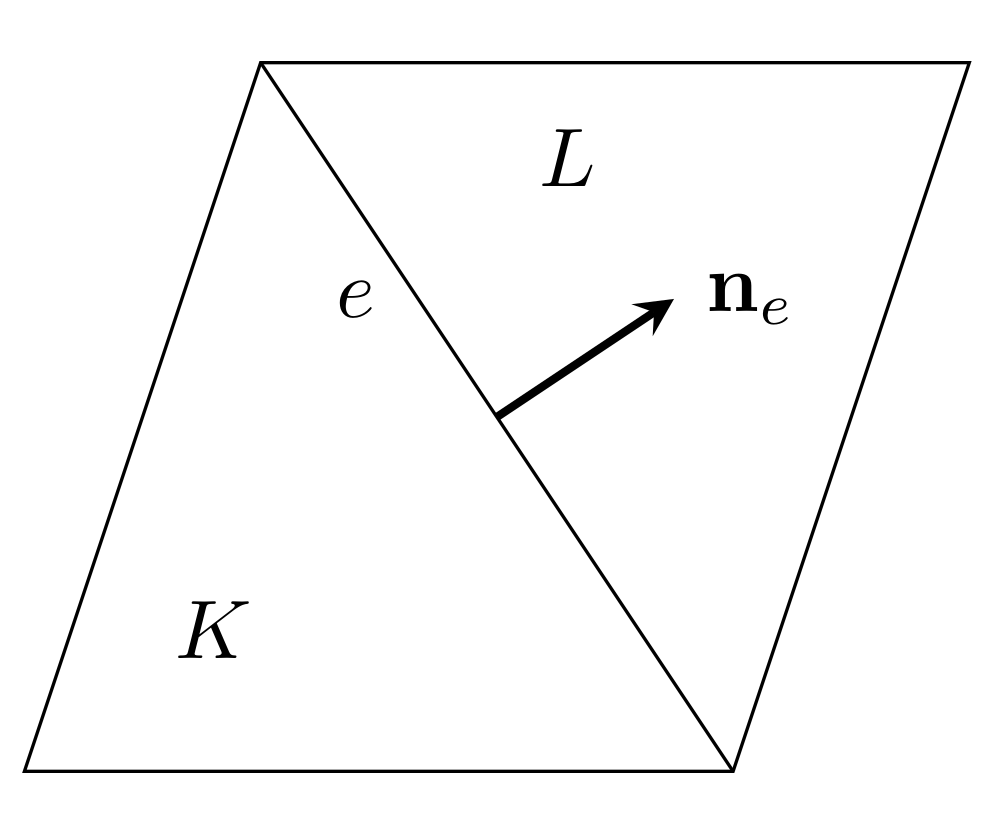
\includegraphics[scale=0.7]{img/figura_tikz.png}
			{\scriptsize\structure{Figure:} Orientation of unit normal vector.}
		\end{figure}
	\end{minipage}
\end{frame}

\begin{frame}{Projection and regularization operators}
	Let $g\in L^1(\Omega)$.

	\begin{itemize}
		\item Projection $\Pi_0\colon L^1(\Omega) \rightarrow \Pd_0(\T_h)$:
		\begin{equation*}
			\escalarL{g}{\overline{w}}=
			\escalarL{\Pi_0 g}{\overline{w}},\forall\,\overline{w}\in \Pd_0(\T_h),
		\end{equation*}
		\item Regularization $\Pi^h_1\colon L^1(\Omega)\rightarrow \Pc_1(\T_h)$
		\begin{equation*}
			\escalarL{g}{\overline{\phi}}=\escalarML{\Pi^h_1 g}{\overline{\phi}},\forall\,\overline{\phi}\in \Pc_1(\T_h),
		\end{equation*}
		where $\escalarML{\cdot}{\cdot}$ is the mass-lumping scalar product in $\Pc_1(\T_h)$
	\end{itemize}
\end{frame}

\begin{frame}{Mesh assumptions}
	\textcolor{red}{Continue}
\end{frame}

\begin{frame}{Nonlinear flux direction}
	\footnotesize
	Notice that
	$$\nabla\cdot(M(u)\nabla\mu)=M'(u)\nabla\mu \cdot\nabla u+M(u)\Delta\mu.$$
	Hence, $\alert{M'(u)}$ determines the direction of the flux.
	
	\vspace*{0.3cm}
	\begin{itemize}
		\item If $u\in[0,1]$ then $M(u)=M(u)_\oplus$.
	\end{itemize}
	\vspace*{0.3cm}
	
	Consider:
	\begin{itemize}
		\item Increasing part of $M(u)_\oplus$: $\alert{M^\uparrow(u)}=
		\begin{cases}
			M(u)_{\oplus} & \text{if }u\le \frac{1}{2}\\[0.2em]
			M\left(\frac{1}{2}\right) & \text{if } u>\frac{1}{2}
		\end{cases}.$
		\item Decreasing part of $M(u)_\oplus$: $
		\alert{M^\downarrow(u)}=
		\begin{cases}
			0 & \text{if }u\le \frac{1}{2}\\
			M(u)_{\oplus}-M\left(\frac{1}{2}\right) & \text{if } u>\frac{1}{2}
		\end{cases}.$
	\end{itemize}
	Notice that $M(u)_\oplus=M^\uparrow(u)+M^\downarrow(u)$.
\end{frame}

\begin{frame}{Generalized upwind method}
	\vspace*{-0.1cm}
	\begin{itemize}\itemsep1em
		\item $a_h^{\text{upw}}:\Pd_k(\T_h)\times \Pd_k(\T_h)\to\R$,
		\begin{multline*}
				\alert{\aupw{\bbeta}{M(u)_\oplus}{\bu}}\coloneqq-\int_\Omega (\bbeta\cdot\nabla\overline{u})M(u)_{\oplus}\\+\sum_{e\in\E_h^i,e=K\cap L}\int_e\left((\media{\bbeta}\cdot\nn_e)_{\oplus}(M^\uparrow(\uK)+M^\downarrow(\uL))\right.\\\left.-(\media{\bbeta}\cdot\nn_e)_{\ominus}(M^\uparrow(\uL)+M^\downarrow(\uK))\right)\salto{\bu},
		\end{multline*}
		where $\bbeta\colon\overline{\Omega}\to\R^d$ can be discontinuous over $\Ehi$.
	\end{itemize}
	
\end{frame}

\subsection{Numerical tests}

\begin{frame}{References}
	\scriptsize 
	\vspace*{-0.25cm}
	\nocite*
	\bibliographystyle{apalike}
	\bibliography{references}
\end{frame}

\begin{frame}{}
	\centering
	\vspace*{1cm}
	{\Huge
		\emph{Thanks for your attention!}}
	
	\vspace*{1cm}
	\begin{acknowledgements}
		The speaker has been supported by a \textit{Graduate Scholarship funded by the University of Tennessee at Chattanooga} and by \textit{UCA FPU contract UCA/REC14VPCT/2020 funded by Universidad de Cádiz}.
		
		The collaborators have been supported by \textit{Grant PGC2018-098308-B-I00} by \textit{MCI N/AEI/ 10.13039/501100011033} and by \textit{ERDF a way of making Europe}.
	\end{acknowledgements}
\end{frame}